\begin{figure}[htb!]
  \centering
  \begin{subfigure}[b]{0.35\textwidth}
    \centering
    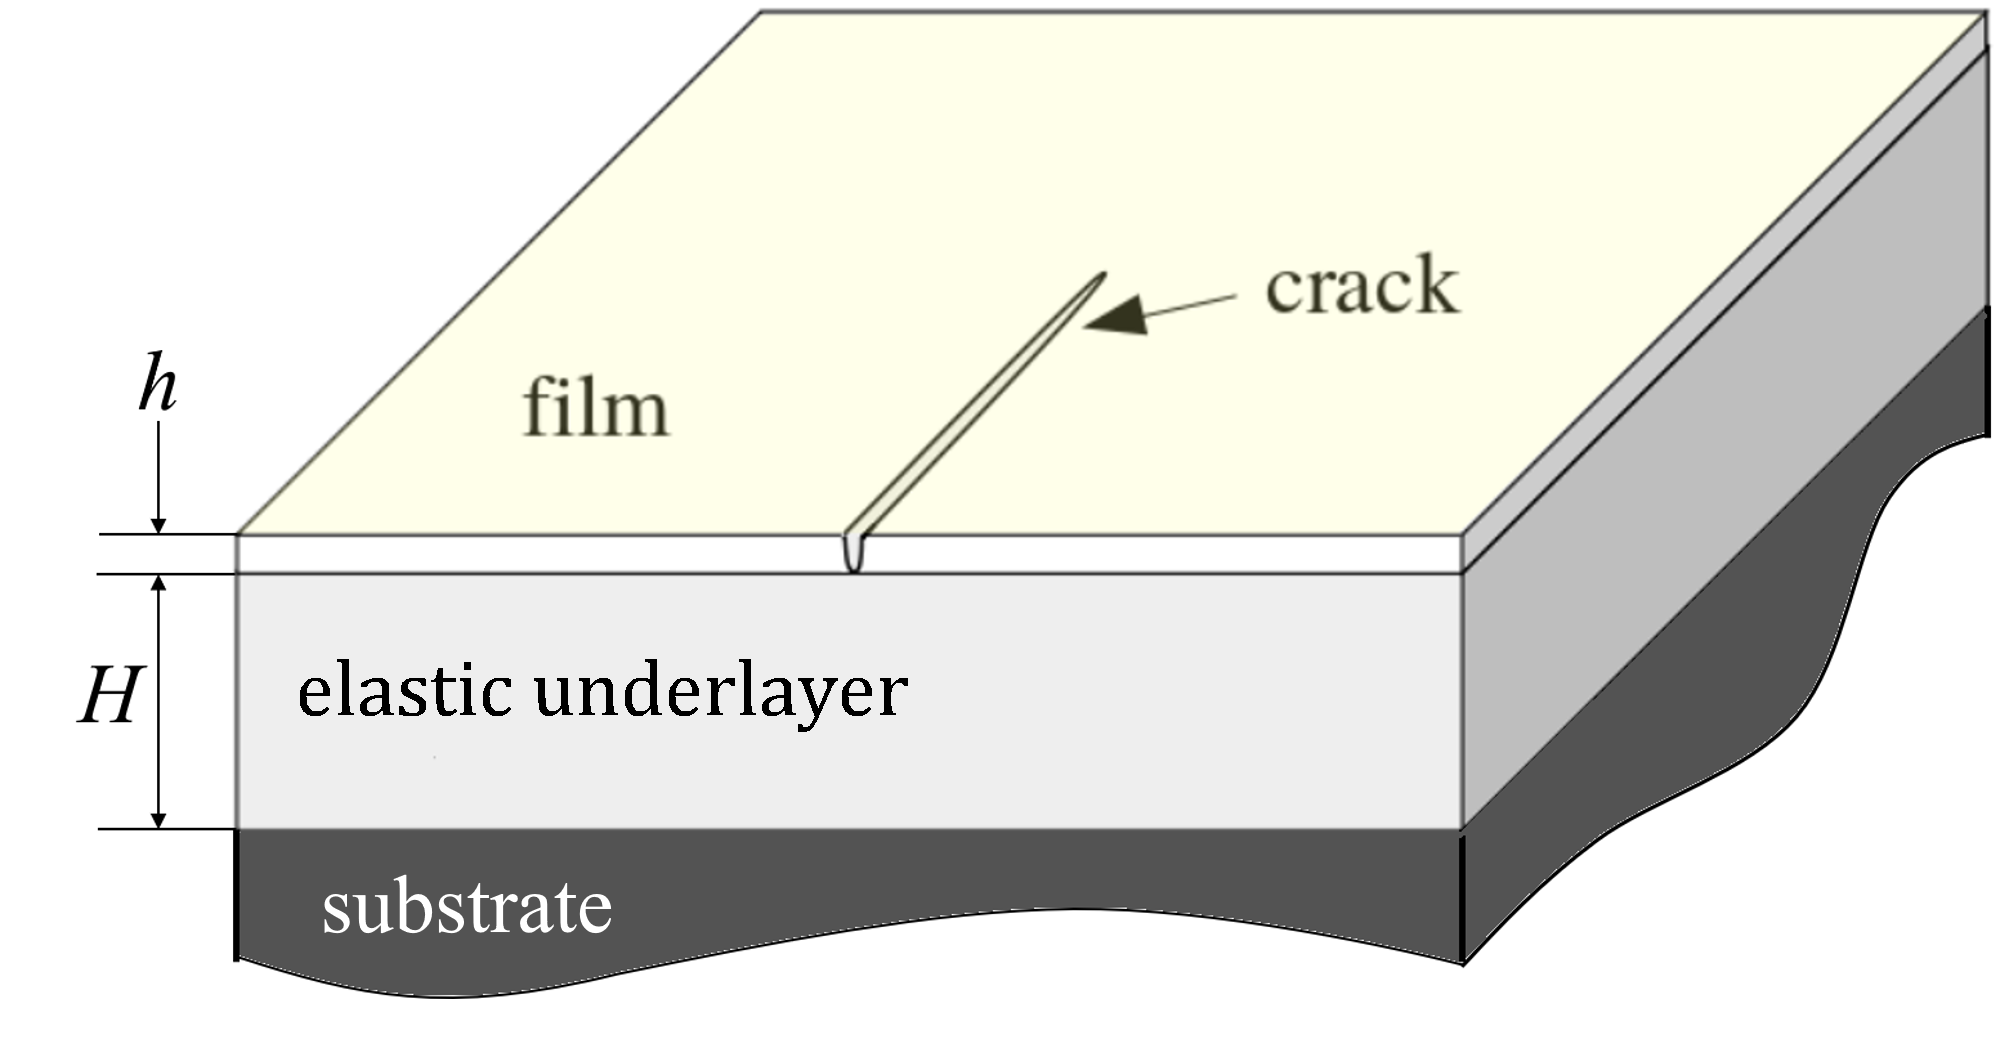
\includegraphics[width=\textwidth,scale=0.5]{Chapter4/figures/2D/top_view.png}
    \caption{}
  \end{subfigure}
  \hspace{0.1\textwidth}
  \begin{subfigure}[b]{0.3\textwidth}
    \centering
    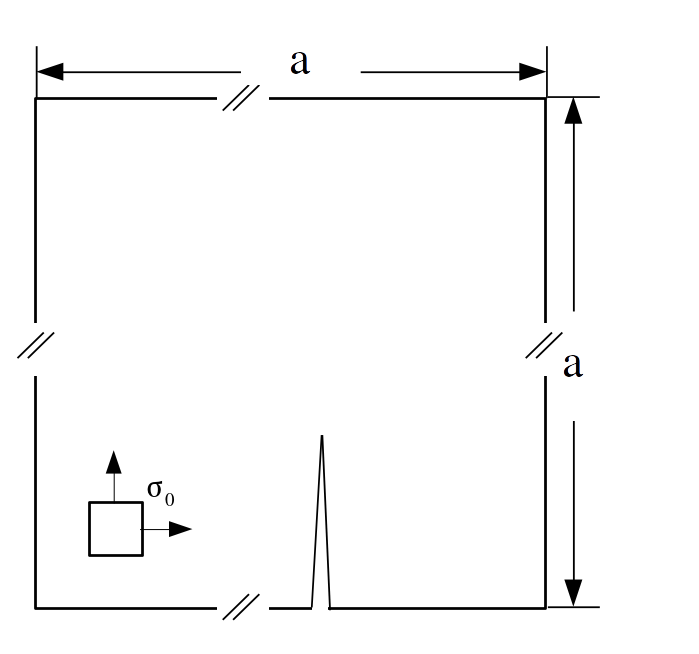
\includegraphics[width=\textwidth,scale=0.5]{Chapter4/figures/2D/2D_schematic.png}
    \caption{}
  \end{subfigure}
  \caption[Description of a two-dimensional model for thin-film cracking.]{Description of a two-dimensional model for thin-film cracking. (a) Top view (highlighted in yellow) (b) schematic representation of the top view. A typical crack is shown to emphasize that fracture is only considered in the film. }
  \label{fig: Chapter4/2D/simplification}
\end{figure}
